\chapter{Estimation of Branching Ratios}
\label{chap:br}
\chapquote{If enough data is collected, anything may be proven by statistical methods.}{Williams and Holland's Law, from Arthur Bloch's book \textit{Murphy's Law}.}
With the available dataset and the established fit model we transform the measured yields of \decay{\Lb}{\Dz\Lz} and \decay{\Xibz}{\Dz\Lz} decays into branching ratios.
In Sec.~\ref{sec:br_Lb} we determine the branching fraction of \decay{\Lb}{\Dz\Lz} w.r.t.\ the three-body decay \decay{\Lb}{\Dz\proton\pim} and discuss systematic uncertainties.
In Sec.~\ref{sec:br_Xib} we then determine the branching ratio of the \Xibz decay w.r.t.\ its \Lb counterpart which can be directly extracted from the fit.
Since the \Xibz yield has a low significance we estimate two-sided confidence intervals and upper limits for this ratio.

\section{Branching Ratio \texorpdfstring{$\BR(\decay{\Lb}{\Dz\Lz}) / \BR(\decay{\Lb}{\Dz\proton\pim})$}{B(Λb → DΛ) / B(Λb → Dpπ)}}
\label{sec:br_Lb}
The data sample used for extracting the signal significances in the previous chapter was an admixture of \gls{lzero} \gls{tis} and \gls{lzero} \gls{tos} triggered events.
Especially for the former, \gls{mc} techniques cannot simulate the efficiency reliably.
For the given dataset the amount of events with a negative \gls{lzero} \gls{tis} trigger decision (\ie{}, only \gls{lzero} \gls{tos} trigger is set) is very low (\cf{}~Fig.~\ref{fig:fit_hLbM_data_LLDD_otos}) and only four such events are found in the signal bin ($5.60 < m(\Dz\Lz) \le 5.64\,\gevcc$).
We argue that excluding those four events by requiring a positive \gls{lzero} \gls{tis} trigger decision does not significantly impact the overall significance, but renders dedicated studies of \gls{lzero} \gls{tos} trigger decisions, that would come with their own set of statistical and systematic uncertainties, needless. 
In contrast to \gls{lzero} \gls{tos} triggered events, the \gls{lzero} \gls{tis} efficiency cancels in good approximation in ratios of decays with common final states, such as \decay{\Lb}{\Dz\Lz} and \decay{\Lb}{\Dz\proton\pim}.
The quality of the approximation even improves, if contributions of non-trivial correlations among the \bquark-hadrons, that were produced during the \proton\proton interaction, cancel in the ratio because they are of the same type (\eg{}, both are \Lb baryons).
Since both conditions are met for \decay{\Lb}{\Dz\Lz} and \decay{\Lb}{\Dz\proton\pim}, we discard events with a negative \gls{lzero} \gls{tis} trigger decision for the estimation of the branching fraction.

Applying the fit in configuration 1 to the reduced data sample yields
\begin{equation*}
    n_\text{TIS}(\decay{\Lb}{\Dz\Lz}) = 28 \pm 7 =
    \begin{cases}
        14 \pm 5 & \text{\gls{LL}}, \\
        14 \pm 5 & \text{\gls{DD}}.
    \end{cases}
\end{equation*}
The projections of this fit for \gls{LL} and \gls{DD} tracks are shown in Fig.~\ref{fig:fit_hLbM_data_fit1_LLDD_tis}.
\begin{figure}[htbp]
    \centering
    \begin{subfigure}[b]{\textwidth}
        \centering
        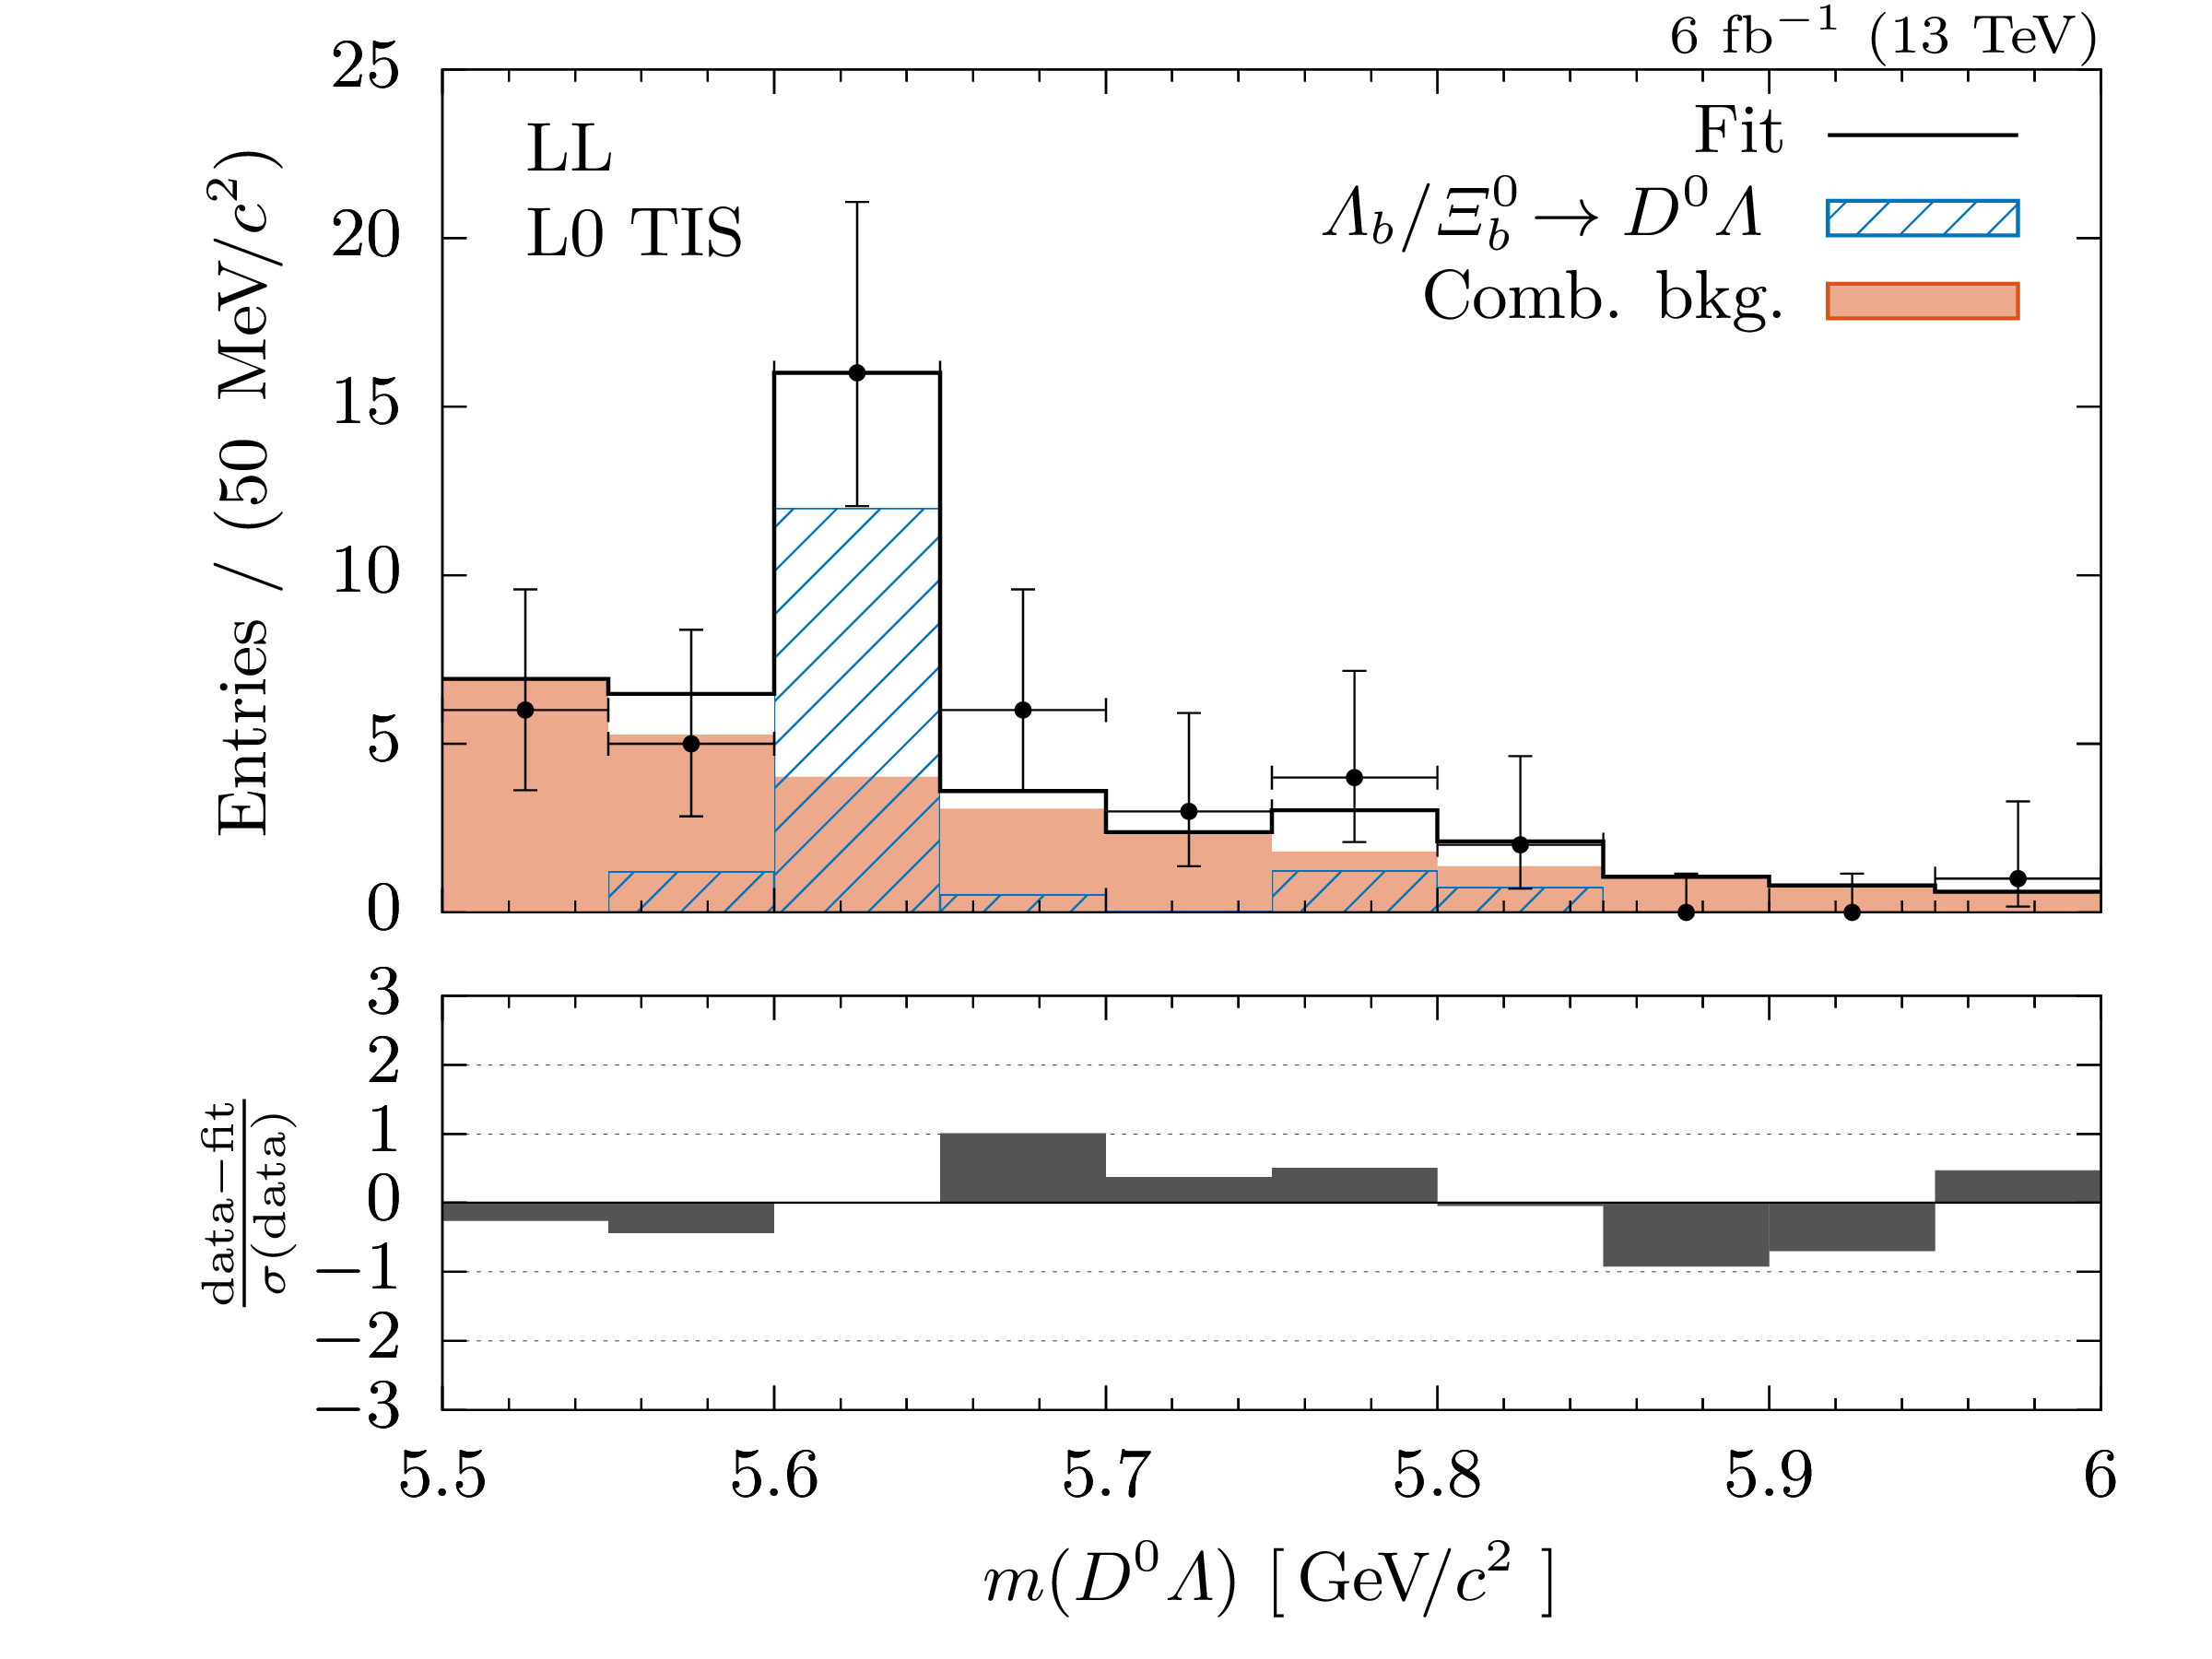
\includegraphics[scale=1.]{fit/hLbM_data_LL_otos-fit.png}
    \end{subfigure}
    \par\bigskip 
    \begin{subfigure}[b]{\textwidth}
        \centering
        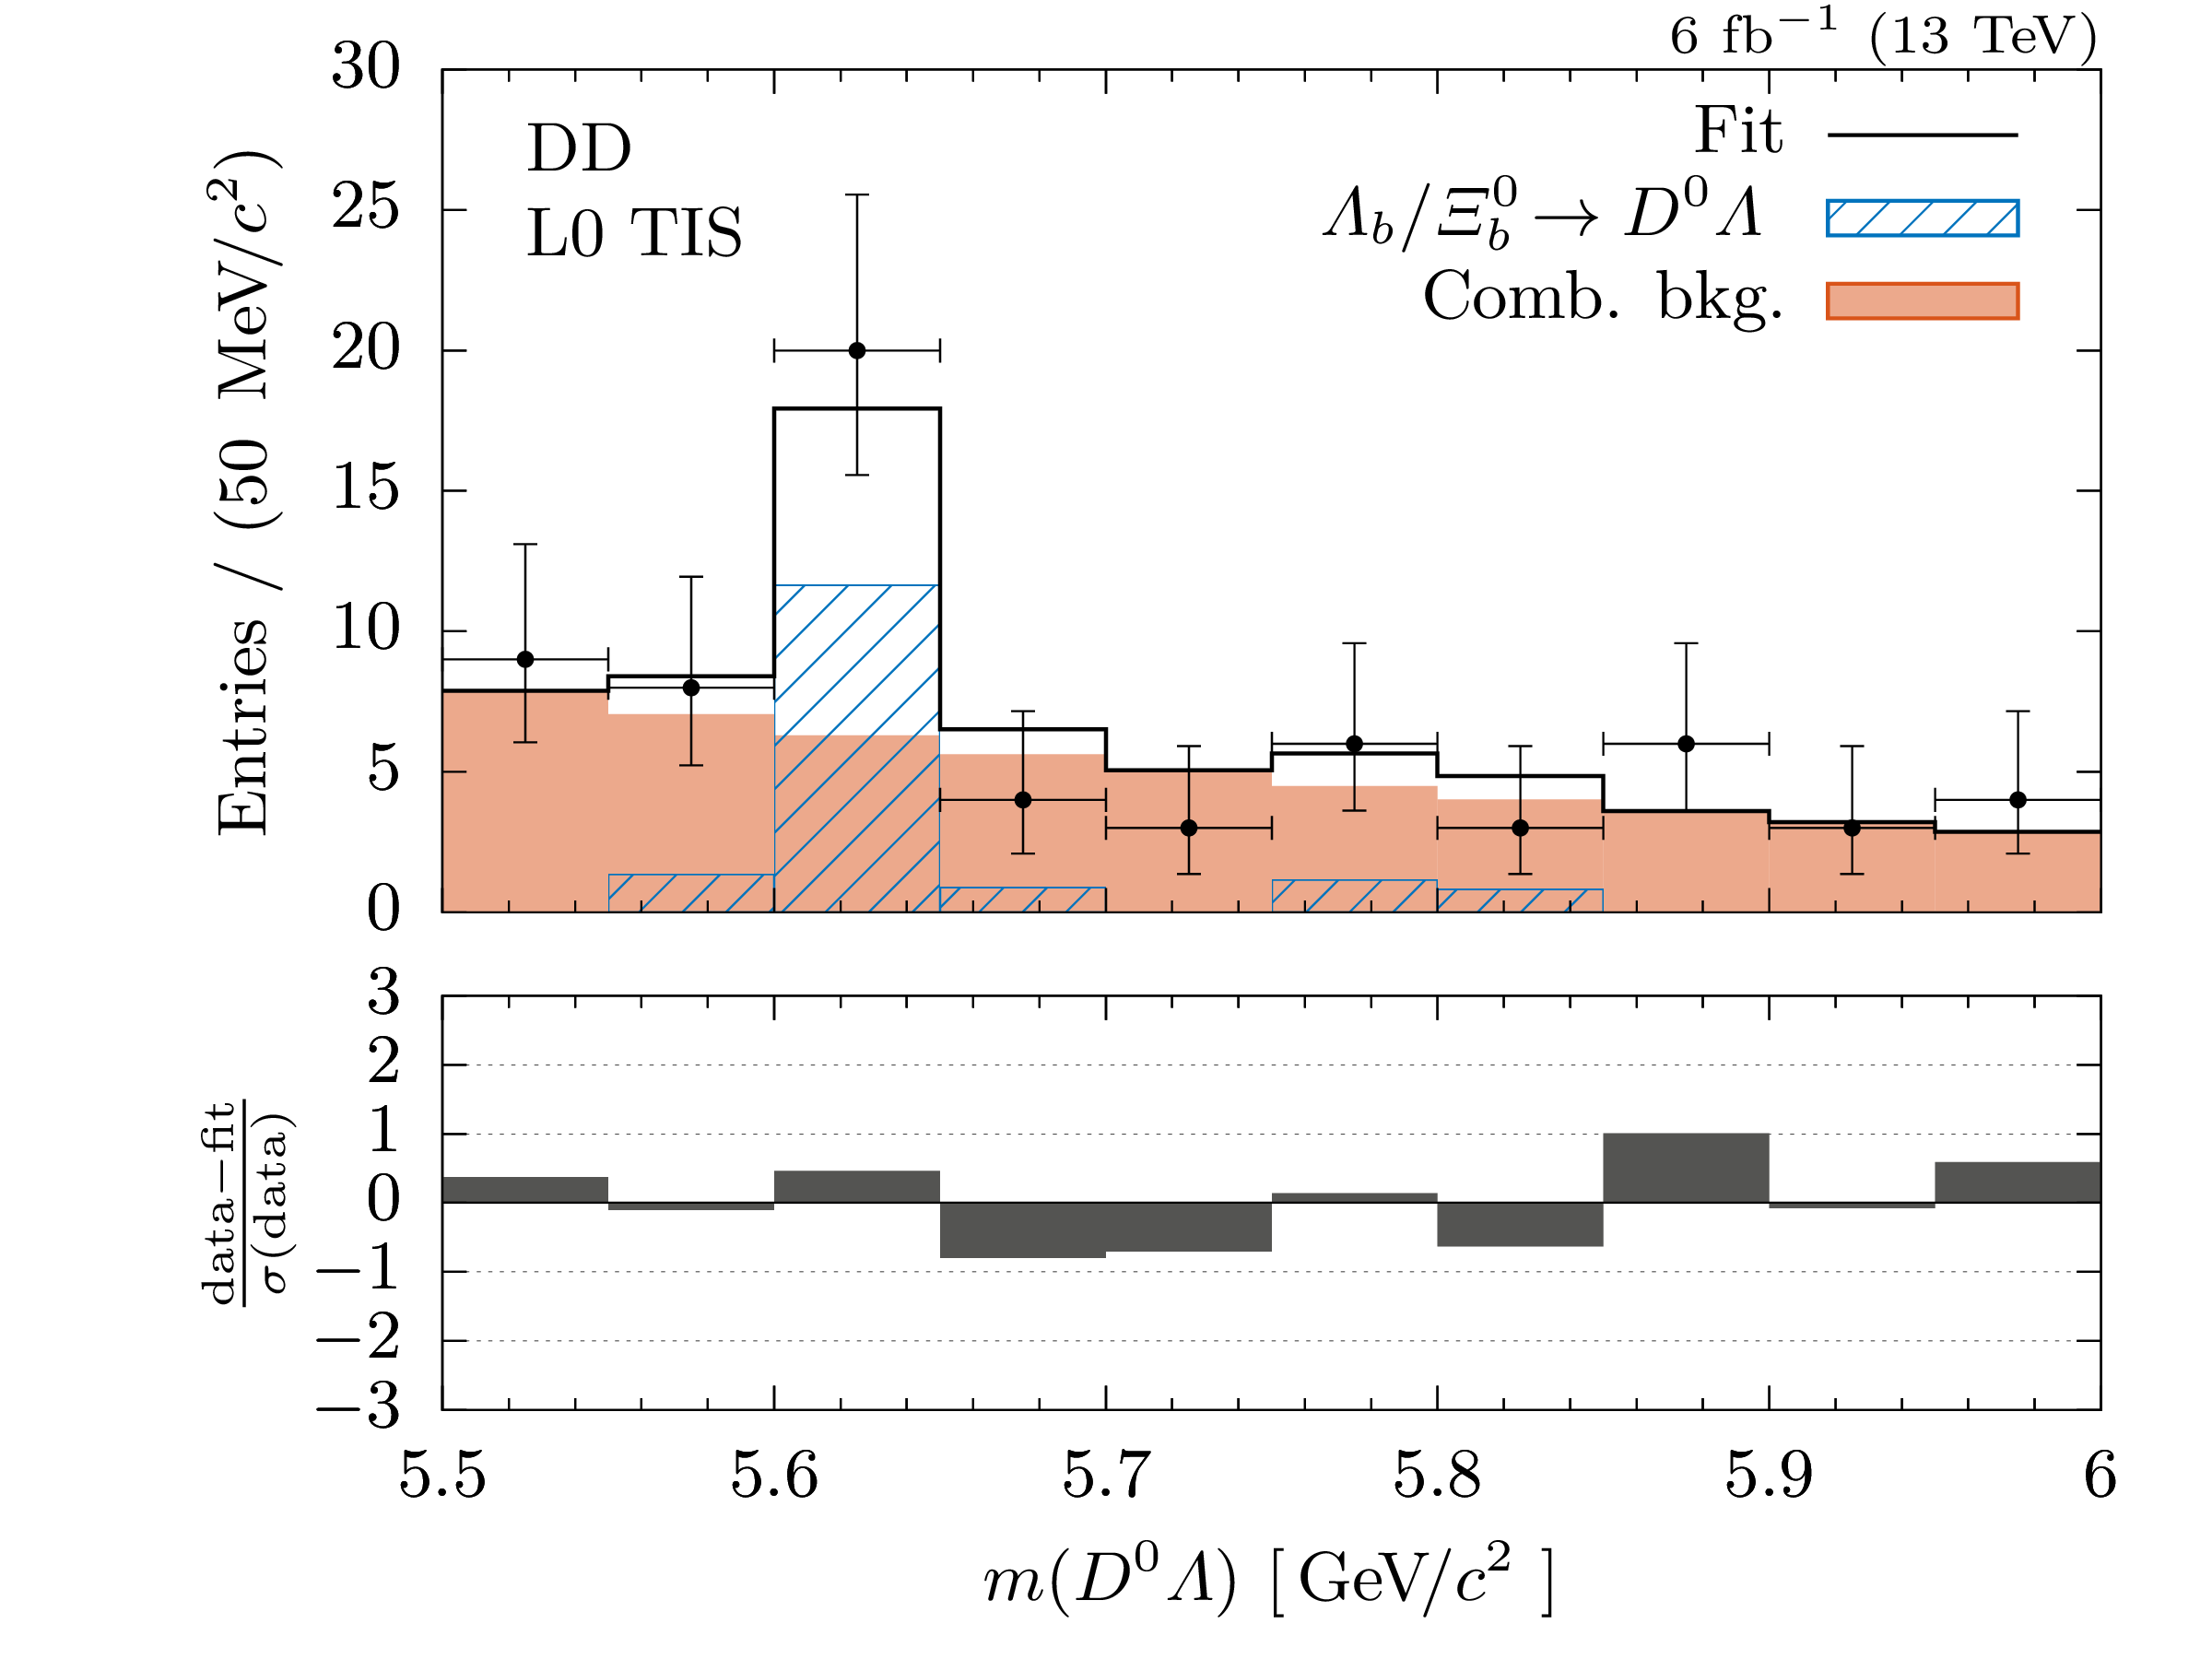
\includegraphics[scale=1.]{fit/hLbM_data_DD_otos-fit.png}
    \end{subfigure}
    \caption{Combined invariant mass of \Dz and \Lz candidates of track type \gls{LL} (top) and \gls{DD} (bottom) from recorded data, as well as the corresponding projections of the simultaneous fit in configuration 1. For recorded data a positive \gls{lzero} \gls{tis} trigger decision is required.}
    \label{fig:fit_hLbM_data_fit1_LLDD_tis}
\end{figure}

The branching ratio is determined by correcting the ratio of the fitted yields by their combined reconstruction and stripping efficiency $\varepsilon_\text{rec\,\&\,strip}$ (\cf{}~Chap.~\ref{chap:stripeff}), the efficiency of the tight selection $\varepsilon_\text{sel}$ and the branching fraction of the \decay{\Lz}{\proton\pim} decay:
\begin{multline*}
    \frac{\BR(\decay{\Lb}{\Dz\Lz})}{\BR(\decay{\Lb}{\Dz\proton\pim})} = 
    \frac{n_\text{TIS}(\decay{\Lb}{\Dz\Lz})}{n_\text{TIS}(\decay{\Lb}{\Dz\proton\pim})} \times 
    \frac{\varepsilon_\text{rec\,\&\,strip}(\decay{\Lb}{\Dz\proton\pim})}{\varepsilon_\text{rec\,\&\,strip}(\decay{\Lb}{\Dz\Lz})} \\
    \times \frac{\varepsilon_\text{sel}(\decay{\Lb}{\Dz\proton\pim})}{\varepsilon_\text{sel}(\decay{\Lb}{\Dz\Lz})} \times
    \frac{1}{\BR(\decay{\Lz}{\proton\pim})} =
    \begin{cases}
        0.015 \pm 0.005 \pm 0.003 & \text{(\gls{LL})}, \\
        0.017 \pm 0.005 \pm 0.004 & \text{(\gls{DD})}, \\
    \end{cases} 
\end{multline*}
where the first (second) error is the total statistical (systematic) uncertainty as the result of an ordinary error propagation.
The components of this propagation are listed in Tab.~\ref{tab:br_uLb} and are discussed below:
\begin{description}
    \item[\decay{\Lb}{\Dz\Lz / \proton\pim} fit] Fitted yields of \gls{lzero} \gls{tis} triggered \decay{\Lb}{\Dz\Lz} and \decay{\Lb}{\Dz\proton\pim} events. The statistical error of the former is dominated by the multinomial part of the fit model. Different variations of this fit model (\cf{}~Sec.~\ref{sec:fit_model}) did not reveal major deviations and we therefore approximate the systematic uncertainty being less than $1:14$ ($<10\,\%$). The total error of the latter is dominated by the systematic uncertainty from the respective fit model (\cf{}~Sec.~\ref{sec:LbToDzppi_yields}).
    \item[$\text{Rec.} \times \text{strip. ratio}$] Ratio of the combined reconstruction and stripping efficiency as derived in Chap.~\ref{chap:stripeff}. The figures are given relative to the total amount of generated \decay{\Lb}{\Dz\Lz} decays and thus also account for the splitting ratio of \decay{\Lz}{\proton\pim} into \gls{LL} and \gls{DD} tracks. The assumed systematic uncertainty of $10\,\%$ is discussed in Chap.~\ref{chap:stripeff}. We note that the statistical uncertainty is correlated among \decay{\Lb}{\Dz\Lz} decays of both track types since both of them use the same sample of \decay{\Lb}{\Dz\proton\pim} candidates for normalization. However, the magnitude of the statistical uncertainties is small compared to the other contributions. Thus they can be neglected.
    \item[\decay{\Lb}{\Dz\Lz / \proton\pim} tight sel.] Efficiency of the tight selection and \decay{\Lb}{\Dz\proton\pim} veto for the former, and efficiency of a subset of the tight selection for the latter, estimated with \gls{mc} simulated events. In order to avoid a potential bias, we use the subset of the available \gls{mc} simulated \decay{\Lb}{\Dz\Lz} decays not used during training (and hyper-parameters optimization) of the classifier at the cost of a slightly larger statistical uncertainty (\cf{}~Sec.~\ref{sec:LbToDzLz_tightsel}). This restriction does not affect the efficiency estimation with \gls{mc} simulated \decay{\Lb}{\Dz\proton\pim} decays since this sample was not involved in the training procedure of the classifiers. The origin of the systematic uncertainties is discussed in Appx.~\ref{chap:apdx_mva_xcheck} and considered a conservative approximation, since parts might cancel in the branching ratio due to the common set of thresholds. The large amount of available \gls{mc} simulated \decay{\Lb}{\Dz\proton\pim} decays yields a small systematic uncertainty which can be neglected (including its correlation) in the context of the full error analysis.
    \item[MC calibration] In Chap.~\ref{chap:weights} we established two different calibration schemes. We use Scheme 2 for the calibration of \gls{mc} simulated events and take the deviation to Scheme 1 as a systematic uncertainty.
\end{description}

\begin{table}[htbp]
    \centering
    \caption{Nominal values ($n$), as well as statistical ($u_\text{stat}$) and systematic ($u_\text{sys}$) uncertainties involved in the estimation of the branching ratio of \decay{\Lb}{\Dz\Lz} and \decay{\Lb}{\Dz\proton\pim} for both track types. Uncertainties which are (partially) correlated among the estimated branching ratios of \gls{LL} and \gls{DD} tracks are marked with $\dagger$.}
    \label{tab:br_uLb}
    \begin{tabular}{lrrrrrr}
        \toprule
        & \multicolumn{3}{c}{\gls{LL}} & \multicolumn{3}{c}{\gls{DD}} \\
        & $n$ & $u_\text{stat}$ & $u_\text{sys}$ & $n$ & $u_\text{stat}$ & $u_\text{sys}$ \\
        \midrule
        \decay{\Lb}{\Dz\Lz} fit (\gls{lzero} \gls{tis}) & $14$ & $31\,\%$ & $<10\,\%$ & $14$ & $33\,\%$ & $<10\,\%$ \\
        \decay{\Lb}{\Dz\proton\pim} fit (\gls{lzero} \gls{tis}) & $\num{39300}$ & $<1\,\%$ & $7\,\%$ & $\num{36000}$ & $<1\,\%$ & $7\,\%$ \\
        $\text{Rec.} \times \text{strip. ratio}^\dagger$ & $17.04$ & $<1\,\%$ & $10\,\%$ & $7.26$ & $<1\,\%$ & $10\,\%$ \\
        \decay{\Lb}{\Dz\Lz} tight sel. & $0.348$ & $2.9\,\%$ & $7\,\%$ & $0.136$ & $6.6\,\%$ & $19\,\%$ \\
        \decay{\Lb}{\Dz\proton\pim} tight sel.${}^\dagger$ & $0.5476$ & $<1\,\%$ & $4.3\,\%$ & $0.5098$ & $<1\,\%$ & $4.9\,\%$ \\
        \gls{mc} calibration & \multicolumn{1}{c}{--} & \multicolumn{1}{c}{--} & $1.9\,\%$ & \multicolumn{1}{c}{--} & \multicolumn{1}{c}{--} & $5.5\,\%$ \\
        $1 / \BR(\decay{\Lz}{\proton\pim})^\dagger$ \cite{pdg} & $1.565$ & \multicolumn{1}{c}{--} & $<1\,\%$ & $1.565$ & \multicolumn{1}{c}{--} & $<1\,\%$ \\
        \midrule
        && $31\,\%$ & $18\,\%$ && $33\,\%$ & $26\,\%$ \\
        \bottomrule
    \end{tabular}
\end{table}

The results for \gls{LL} and \gls{DD} tracks can be combined and averaged to improve the overall significance
\begin{equation*}
    \frac{\BR(\decay{\Lb}{\Dz\Lz})}{\BR(\decay{\Lb}{\Dz\proton\pim})} = 0.016 \pm 0.004 \pm 0.003 \,.
\end{equation*}
Combining the ratio with the measured branching fraction
\begin{equation*}
    \BR(\decay{\Lb}{\Dz\proton\pim}) = (6.3 \pm 0.7) \times 10^{-4} \,,
\end{equation*}
as reported by the \gls{pdg}, yields
\begin{equation}
    \label{eq:br_fracLb}
    \frac{\BR(\decay{\Lb}{\Dz\Lz})}{\BR(\decay{\Lb}{\Dz\proton\pim})} \times \BR(\decay{\Lb}{\Dz\proton\pim}) = (9.9 \pm \underbrace{2.3 \pm 1.6 \pm 1.1}_{3.0}) \times 10^{-6} \,,
\end{equation}
where the first (second) uncertainty is statistical (systematic) and the third error is the (external) uncertainty of the normalization.
The total uncertainty is $3.0 \times 10^{-6}$.
Our result thus is compatible with the theory prediction from Ref.~\cite{brLbToDzLz_pred}
\begin{equation*}
    \BR_\mathrm{pred}(\decay{\Lb}{\Dz\Lz}) = 4.56 \times 10^{-6}
\end{equation*}
within two standard deviations.
We note that the measurement of $\BR(\decay{\Lb}{\Dz\proton\pim})$, although dominated by an \lhcb measurement, is not correlated with our measurement since the \lhcb analysis uses data recorded during \gls{runone} rather than \gls{runtwo} as we do in the present analysis~\cite{pdg,LbToDzphAndLch}.

\section{Branching Ratio \texorpdfstring{$\BR(\decay{\Xibz}{\Dz\Lz}) / \BR(\decay{\Lb}{\Dz\Lz})$}{B(Ξb → DΛ) / B(Λb → DΛ)}}
\label{sec:br_Xib}
The constraint fit to the combined invariant mass of \Dz and \Lz candidates of both track types allows a clean extraction of the branching ratio 
\begin{equation}
    \label{eq:br_XibLb_ratio_theo}
    \frac{\BR(\decay{\Xibz}{\Dz\Lz})}{\BR(\decay{\Lb}{\Dz\Lz})} = \frac{f_{\Lb}}{f_{\Xibz}} \times \frac{1 - f_s}{f_s},
\end{equation}
where $f_{\Lb} / f_{\Xibz}$ is the ratio of the fragmentation fractions of $\bquark$-quarks into \Lb and \Xibz baryons, and $f_s$ is a fit parameter that we established in Sec.~\ref{sec:fit_model}. (Not to be confused with the fragmentation fractions of $\bquark$-quarks into \Bs mesons.)
The systematic uncertainty of this technique is very low in comparison to the large statistical uncertainty.
Fidelity issues in \gls{mc} simulated events play a minor role and enter only if they induce a non-trivial correction to the ratio Eq.~\eqref{eq:br_XibLb_ratio_theo} which is disfavored by the \gls{mc} simulated \decay{\Lb}{\Dz\Lz} and \decay{\Xibz}{\Dz\Lz} decays (\cf{}~Tab.~\ref{tab:fit_ndatasamples}).
In particular we find that the nominal value of the branching ratio is largely independent of our choice of the \gls{mc} calibration.

We estimate two confidence intervals (CI) following a frequentist interpretation by using pseudo-experiments, and two CIs using a Bayesian interpretation by scanning the fitted likelihood profiles of $f_s$ and assuming a uniformly distributed prior $(1 - f_s) / f_s$.
All these intervals are shown in Fig.~\ref{fig:br_xiblb_brs} and Tab.~\ref{tab:br_xiblb_brs} with $68\,\%$ and $90\,\%$ CL.
(We note that the upper boundary of the two-sided \textit{shortest} CIs (in both interpretations) with a $90\,\%$ CL are equivalent to $95\,\%$ CL upper limits.)
We also estimate a Bayesian upper limit when requiring a minimal flight distance significance of \Dz candidates to suppress charmless \Xibz backgrounds (\cf{}~Sec.~\ref{sec:bkgs_charmless}) and append the result to Tab.~\ref{tab:br_xiblb_brs}.
In Appx.~\ref{chap:apdx_brxiblb} we give a more detailed overview about the estimation of these CIs.
\begin{figure}[htbp]
    \centering
    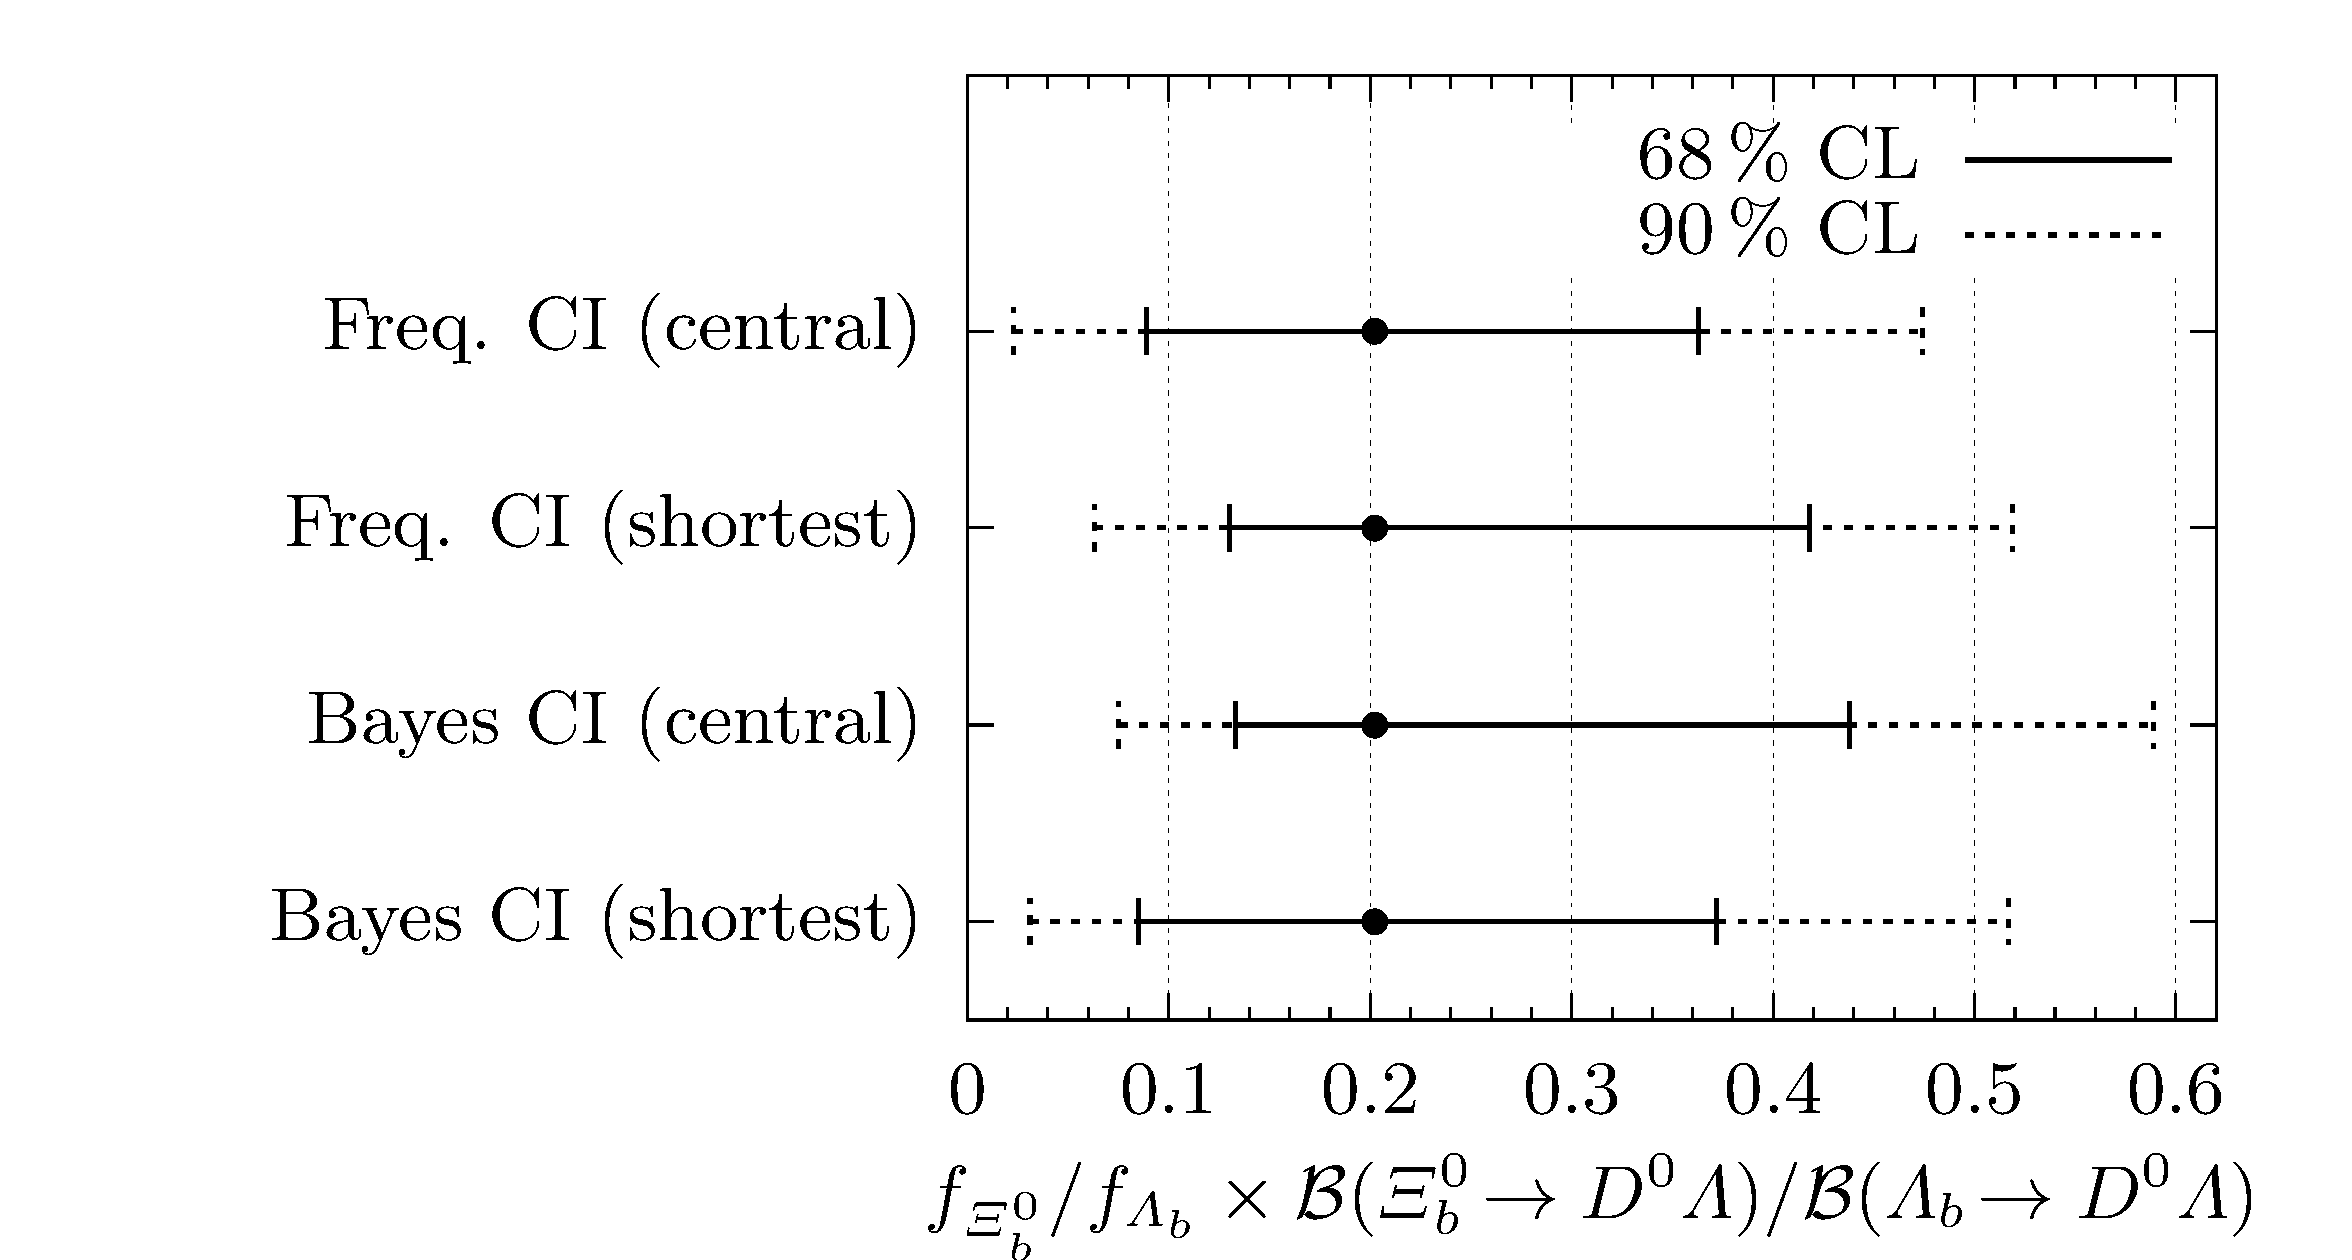
\includegraphics[scale=1.]{br/xiblb_brs.png}
    \caption{Two-sided CIs with 68\,\% and 90\,\% coverage for $(1 - f_s) / f_s$, estimated using different frequentist and Bayesian approaches. We note that the upper boundaries of the (two-sided) central CIs with 90\,\% CL are identical with 95\,\% CL upper limits.}
    \label{fig:br_xiblb_brs}
\end{figure}

\begin{table}[htbp]
    \centering
    \caption{Two-sided CIs with 68\,\% and 90\,\% coverage, as well as 95\,\% CL upper limits for $(1 - f_s) / f_s$, estimated using different frequentist and Bayesian approaches. The limits shown in the last row ($\dagger$) are the results of a fit when an additional veto against charmless \Xibz backgrounds is required.}
    \label{tab:br_xiblb_brs}
    \begin{tabular}{llll}
        \toprule
        Method & \multicolumn{1}{c}{68\,\% CL} & \multicolumn{1}{c}{90\,\% CL} & \multicolumn{1}{c}{95\,\% CL} \\
        \midrule
        Freq. CI (central) & $[0.089 \, \ldots \, 0.363]$ & $[0.023 \, \ldots \, 0.474]$ & $[0 \, \ldots \, 0.474]$ \\
        Freq. CI (shortest) & $[0.130 \, \ldots \, 0.418]$ & $[0.063 \, \ldots \, 0.519]$ & \multicolumn{1}{c}{--} \\
        Bayes CI (central) & $[0.133 \, \ldots \, 0.438]$ & $[0.075 \, \ldots \, 0.589]$ & $[0 \, \ldots \, 0.589]$ \\
        Bayes CI (shortest) & $[0.085 \, \ldots \, 0.372]$ & $[0.031 \, \ldots \, 0.517]$ & \multicolumn{1}{c}{--} \\
        Bayes CI (upper limit${}^\dagger$) & \multicolumn{1}{c}{--} & $[0 \, \ldots \, 0.437]$ & $[0 \, \ldots \, 0.537]$ \\
        \bottomrule
    \end{tabular}
\end{table}

The measurements of absolute branching fractions are difficult to perform at hadron colliders without using external input.
In particular, measurements of absolute \Xib branching fractions are limited by the amount of available data, thus it is still common to report branching ratios involving \Xib baryons in product with the respective \bquark-fragmentation ratios.
Lately, first indirect measurements of $f_{\Xibz}/f_{\Lb}$ were carried out by the \lhcb collaboration~\cite{fXibzfLb} and leveraged the predictions $f_{\Xibz}/f_{\Lb} = 0.065(20)$~\cite{fXibzfLb_theo1} and $f_{\Xibz}/f_{\Lb} = 0.054(20)$~\cite{fXibzfLb_theo2}.
Still, it is known from precise measurements of \bquark-fragmentations into different \bquark-mesons and \Lb baryons that these values depend on transverse momentum and pseudo-rapidity~\cite{LHCb_bProdFrac_7,LHCb_bProdFrac_13}.
A first measurement of $f_{\Xibm}/f_{\Lb}$ at different center-of-mass energies confirms this dependence for \Xib baryons~\cite{fXibmfLb}.
Since measurements and predictions of $f_{\Xibz}/f_{\Lb}$ are still rare and kinematic dependencies are not yet included in the predictions, we stick to the common practice and only report the product of the branching fraction $\BR(\decay{\Xibz}{\Dz\Lz}) / \BR(\decay{\Lb}{\Dz\Lz})$ and the fragmentation ratio $f_{\Xibz}/f_{\Lb}$.

\section{Summary and Outlook}
%\chapquote{Prediction is very difficult, especially if it's about the future.}{Niels Bohr, physicist and Nobel laureate.}
Using the full available \gls{runtwo} data set we find the decay \decay{\Lb}{\Dz\Lz} with a statistical significance of $5.5$ standard deviations and estimate the branching ratio
\begin{equation}
    \label{eq:br_Lbbr}
    \frac{\BR(\decay{\Lb}{\Dz\Lz})}{\BR(\decay{\Lb}{\Dz\proton\pim})} = 0.016 \pm 0.004 \pm 0.003 \,,
\end{equation}
where the first uncertainty is statistical and the second is systematic.
An excess of \decay{\Xibz}{\Dz\Lz} candidates is observed with a statistical significance of $1.8$ standard deviations and used to estimate upper limits, \eg{},
\begin{equation}
    \label{eq:br_Xibzbr}
    \frac{f_{\Xibz}}{f_{\Lb}} \times \frac{\BR(\decay{\Xibz}{\Dz\Lz})}{\BR(\decay{\Lb}{\Dz\Lz})} < 0.5 \quad (\text{CL} = 95\,\%) \,.
\end{equation}
Let us recap how these results were obtained:
In Chap.~\ref{chap:weights} we calibrated \gls{mc} simulated events and used them together with recorded data to train binary classifiers in Chap.~\ref{chap:mva} to separate signal and combinatorial background.
Contributions from physical backgrounds were analyzed in Chap.~\ref{chap:bkgs} and were either found negligible after requiring dedicated selections or were included in the fit model described in Chap.~\ref{chap:fit}.
Studies of the normalization mode were presented in Chap.~\ref{chap:norm}.

The results reported in Eq.~\eqref{eq:br_fracLb}, Eq.~\eqref{eq:br_Lbbr}, and Eq.~\eqref{eq:br_Xibzbr} are limited statistically, even though the intermediate particles are reconstructed in their dominant modes, \ie{}, \decay{\Dz}{\Km\pip} and \decay{\Lz}{\proton\pim}.
The inclusion of more decay modes, for example \decay{\Dz}{\Km\pip\pip\pim}, can increase the significances slightly and allow \CP measurements.
However, to actually measure \gls{ckm} parameters, at least the Cabibbo suppressed decays \decay{\Dz}{\Km\Kp} and \decay{\Dz}{\pim\pip} have to be reconstructed, corresponding to the requirement of roughly $1 / \lambda^2 \approx 20$ times more data.
This is in reach within the next runs of the \lhc.
Additionally, charmless \Lb decays will enter into these modes as non-resonant background and require rich statistics to control, for example by analyzing the lifetime of \Dz candidates.

A sufficiently large data sample which would allow the reconstruction of the Cabibbo doubly suppressed modes \decay{\Dz}{\Kp\pim}, would not just leverages an extraction of the \gls{ckm} parameter $\gamma$ using \gls{ads} and \gls{glw} methods in decays of baryons, but would also allow a clean extraction of $\BR(\decay{\Xibz}{\Dz\Lz})$ due to the absence of charmless backgrounds in this mode.
On top, an extraction of \Sz modes (both in \Lb and \Xibz) similar to Ref.~\cite{IsospinInLbToJpsiLz} would become feasible and thus would allow inference of yet unseen modes such as \decay{\Xibz}{\Dz\Xiz} or \decay{\Lb}{\Dz\neutron}.
